\documentclass[12pt, a4paper]{article}
\usepackage[utf8]{inputenc}
\usepackage[english, russian]{babel}
\usepackage{indentfirst}
\usepackage{misccorr}
\usepackage{graphicx}
\usepackage{amsmath}
\usepackage{graphicx}
\usepackage{float}
\usepackage{url}
\usepackage{subfigure}
\usepackage[hidelinks]{hyperref}
\usepackage[left=20mm,right=10mm, top=20mm,bottom=20mm,bindingoffset=0mm]{geometry}
\setlength{\parindent}{2em}
\setlength{\parskip}{6pt}\graphicspath{{images/}}\DeclareGraphicsExtensions{.png}


\begin{document}
\begin{titlepage}
\begin{center}

\large
Санкт-Петербургский политехнический университет\\Петра Великого\\
\vspace{0.5cm}
Физико-механический институт\\
\vspace{0.25cm}
Высшая школа прикладной математики и вычислительной физики
\vfill
\textsc{\large\textbf{Отчет по лабораторной работе}}\\[2cm]
\large
по дисциплине\\"Механика жидкости и газа"
\end{center}
\vfill
\begin{tabular}{l p{280} l}
            Выполнил студент\\Группы 5030102/90101 && Можаев А.А.
            \vspace{0.25cm}
            \\Руководитель: && Синицина Д.Э.
        \end{tabular}
        \vfill
        \begin{center}
            Санкт-Петербург\\2022 г.
        \end{center}
\end{titlepage}

\newpage
\begin{center}
    \tableofcontents
    \setcounter{page}{2}
\end{center}

\newpage
\begin{center}
    \listoffigures
\end{center}

\newpage
\begin{center}
    \listoftables
\end{center}

\newpage
\section{Лабораторная работа №1}
\subsection{Постановка задачи}
При анализе результатов расчетов следует (для всех рассмотренных значений Re):
\begin{itemize}
    \item 
        Проанализировать векторные поля скорости и скалярные распределения компонент скорости, проиллюстрировать изменение профиля скорости от входного к характерному для участка развитого течения.
    \item
        Оценить длину начального участка канала (в качестве границы начального участка следует выбрать сечение, в котором значение максимальной скорости составляет $98\%$ от максимальной скорости развитого течения $V_{max}$ = 1.5$V_{вх}$); провести сопоставление полученных результатов по длине начального участка с аналитическим решением $\frac{L_{нач}}{H} = 0.04 \cdot Re$; представить результаты в виде таблицы и графически.
    \item
        Проанализировать поле нормированного давления; найти коэффициент сопротивления $\lambda$ для участка с установившимся параболическим профилем скорости при помощи формулы 
        \begin{equation}
            \Delta p = \lambda \frac{\Delta L \rho v_{ср}^2}{2H}
        \end{equation}
        где $\Delta p$ – перепад давления на участке канала длиной $\Delta L$, $\rho$ = const – плотность жидкости, $V_{ср}$ – средняя по сечению скорость, за масштаб давления в рассматриваемой постановке задачи принимается величина $\rho V_{вх}^2$, где $V_{вх}$ – модуль скорости на входе. Определить значение $\lambda$ для участка развитого течения из угла наклона линейного участка зависимости. Провести сопоставление с теоретической оценкой для развитого участка $\lambda$ = 24/Re; представить результаты в виде таблицы и графически.
    \item
        Построить график зависимости коэффициента трения на стенке канала, $C_f$, от координаты x. Одномерное распределение коэффициента трения следует экспортировать в формате Tecplot, вызвав визуализатор распределений физических величин по границам, четыре зоны в получающемся при экспорте данных plt-файле соответствуют четырем границам расчетной области, коэффициент трения экспортируется в Tecplot под названием «Skin Friction». Проанализировать распределение коэффициента трения и убедиться в том, что для участка развитого течения выполняется соотношение  $\lamda = 2C_f$.
\end{itemize}

\subsection{Реализация}
Лабораторная работа выполнена с помощью встроенных средств Tecplot, Flos.

\subsection{Результаты}

\subsubsection{Векторное поле скорости}
\begin{figure}[H]
    \centering
    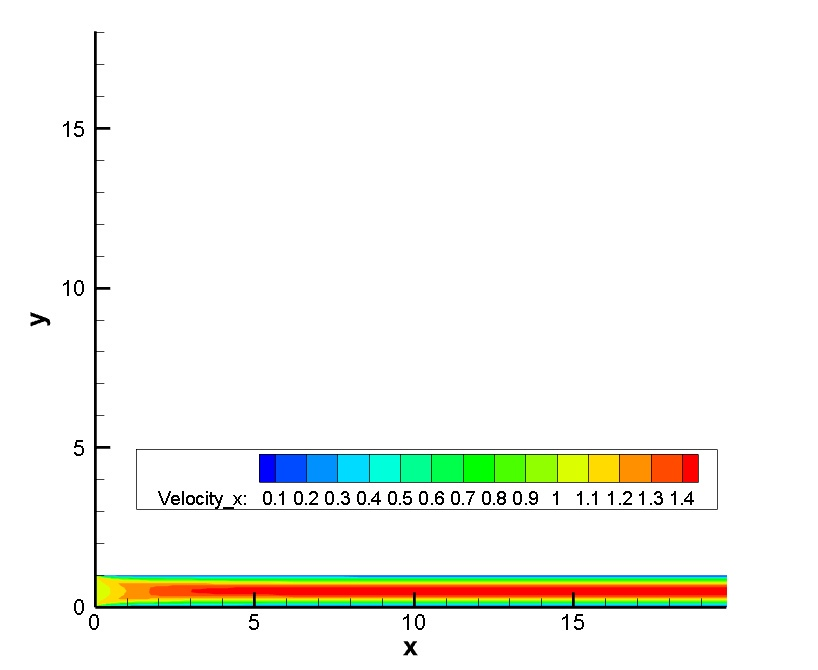
\includegraphics[scale = 0.8]{figure/RE135_Velocity_x.jpg}
    \caption{Поле скалярной скорости, зависящей от x для RE=435}
    \label{pic1}
\end{figure}

\begin{figure}[H]
    \centering
    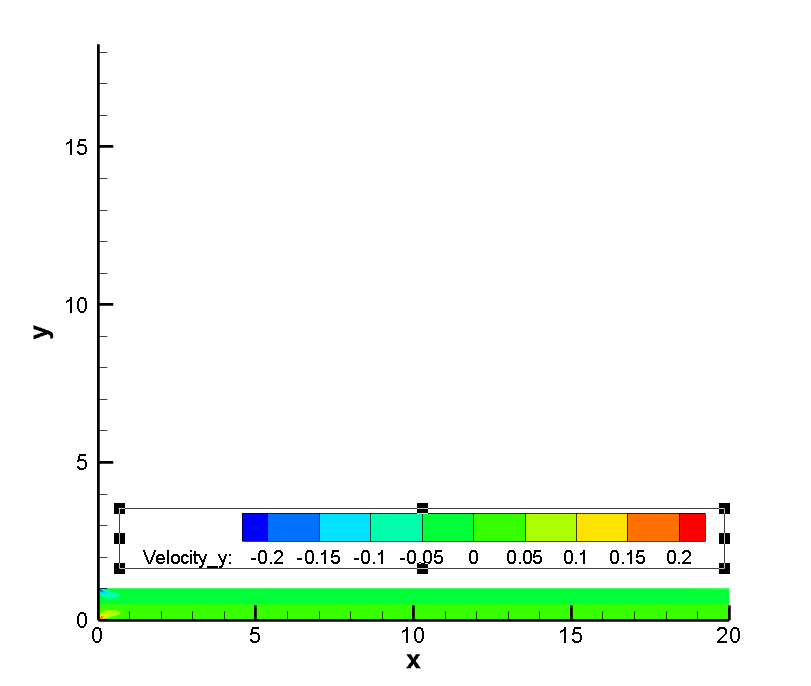
\includegraphics[scale = 0.8]{figure/RE135_Velocity_y.png}
    \caption{Поле скалярной скорости, зависящей от y для RE=435}
    \label{pic2}
\end{figure}

\begin{figure}[H]
    \centering
    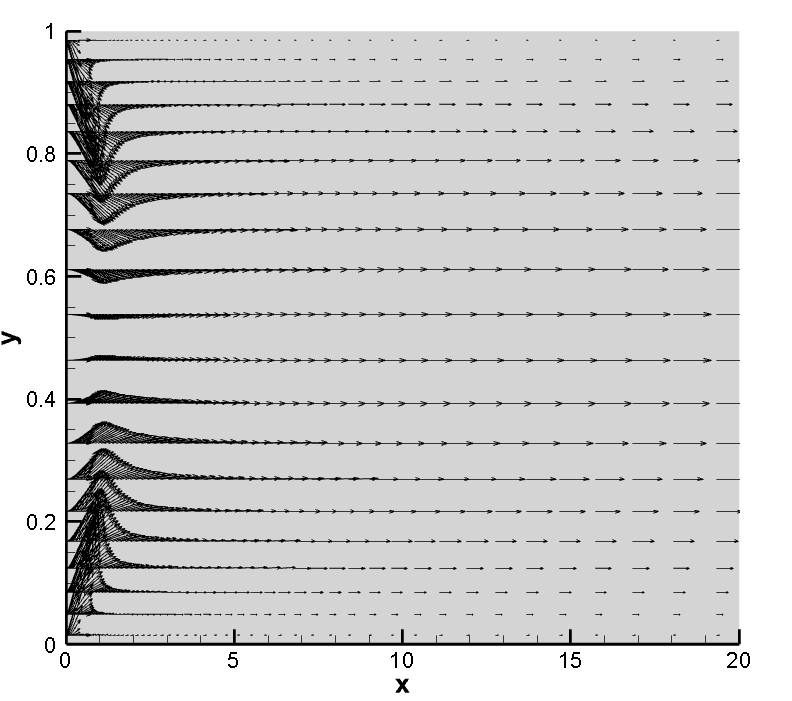
\includegraphics[scale = 0.6]{figure/RE135_vector.png}
    \caption{Поле векторной скорости для RE=435}
    \label{pic3}
\end{figure}

\begin{figure}[H]
    \centering
    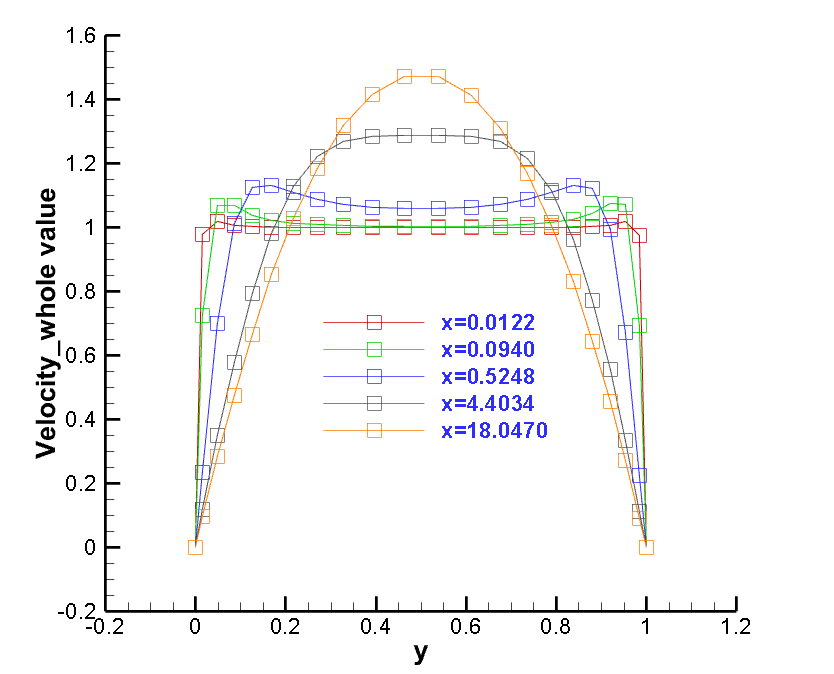
\includegraphics[scale = 0.6]{figure/RE135_speed.png}
    \caption{Характеристики профиля скорости от x}
    \label{pic4}
\end{figure}

\subsubsection{Начальный участок канала}

\begin{figure}[H]
    \centering
    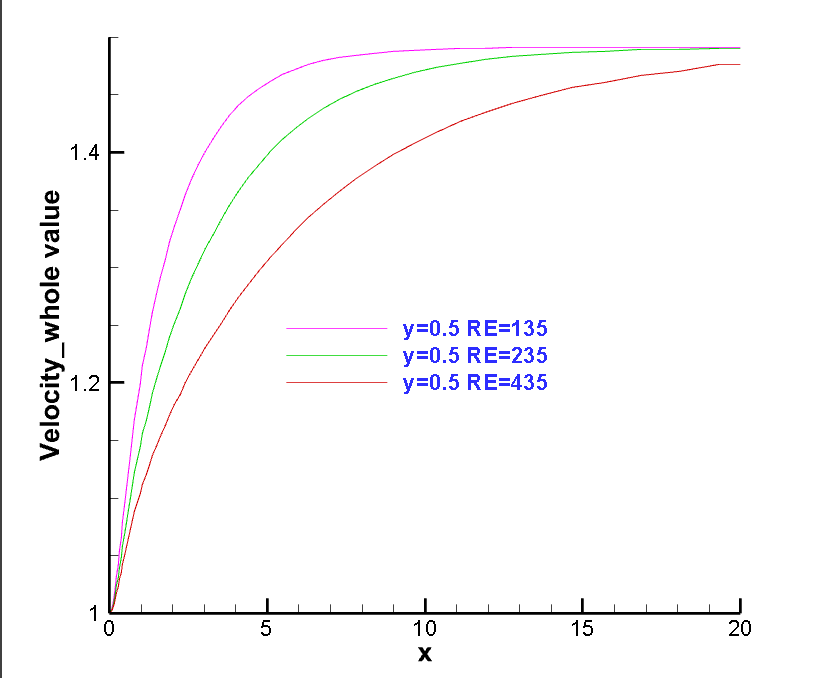
\includegraphics[scale = 0.6]{figure/y=0.5_RE=all.png}
    \caption{Длина начального участка при Re = 135,235,435}
    \label{pic5}
\end{figure}


\begin{table}[H]
    \centering
    \begin{tabular}{|c|c|c|c|}
    \hline
        Re  &  $L_{\text{нач}}$  &  $L_{\text{анал}}$  &  погр(\%) \\
    \hline
        135  &  5.731  &  5.4  &  6.13\\
    \hline
        235	 &  9.756  &  9.4  &  3.79\\
    \hline
        435  &  17.9  &  17.4  &  2.87\\
    \hline
    \end{tabular}
    \caption{Таблица начальных участков в сопоставлении с аналитическими}
    \label{Tab1}
\end{table}

\subsubsection{Поле нормированного давления}
\begin{figure}[H]
    \centering
    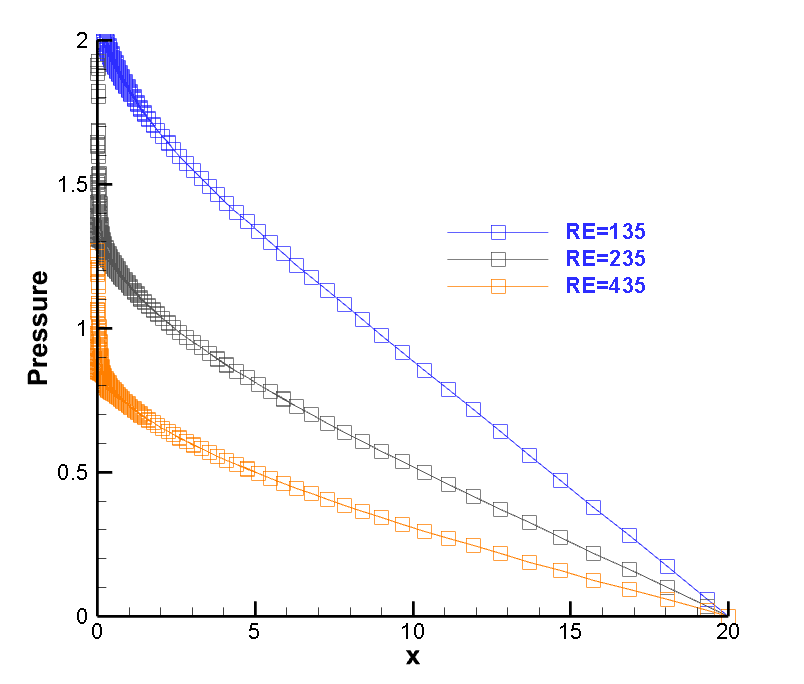
\includegraphics[scale = 0.6]{figure/pressure_RE=all.png}
    \caption{Поле нормированного давления }
    \label{pic9}
\end{figure}

\begin{table}[H]
    \centering
    \begin{tabular}{|c|c|c|c|c|c|c|}
    \hline
        Re  &  $\lambda$  &  $\lambda_{\text{анал}}$  &  погр(\%) \\
    \hline
        135  &  0.17399 &  0.17778  &  2.131\\
    \hline
        235	 &  0.09666  &  0.10213	 &  5.356\\
    \hline
        435  &  0.06053  &  0.05517  &  8.855\\
    \hline
    \end{tabular}
    \caption{Таблица коэффициентов сопротивления в сопоставлении с аналитическими}
    \label{tab2}
\end{table}

\subsubsection{Коэффициент трения}
\begin{figure}[H]
    \centering
    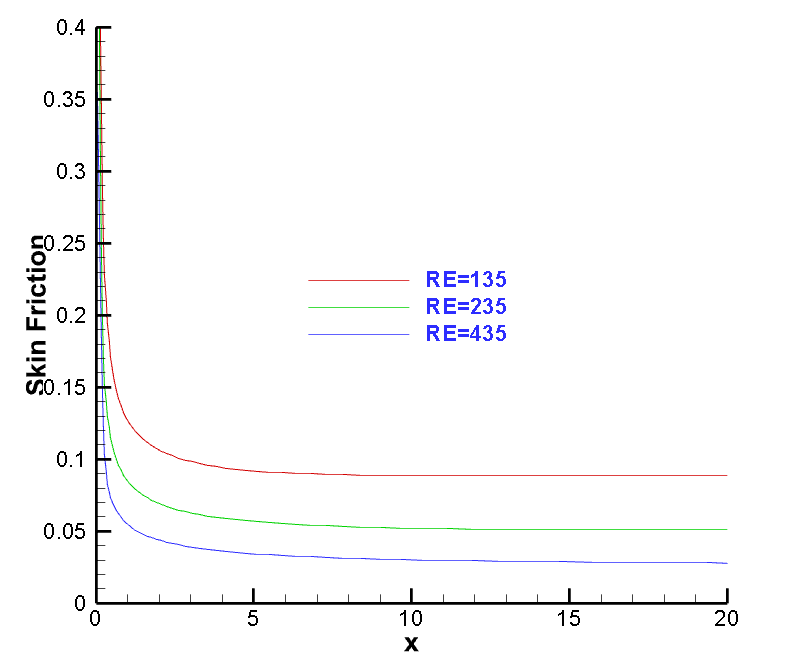
\includegraphics[scale = 0.6]{figure/SkinFriction_RE=all_1.png}
    \caption{Коэффициент трения}
    \label{pic10}
\end{figure}

\begin{table}[H]
    \centering
    \begin{tabular}{|c|c|c|c|}
    \hline
        Re  &  $C_f$  &  $C_f\_{\text{анал}}$  &  погр(\%)\\
    \hline
        135  &  0.08866  &  0.08889  &  0.25829\\
    \hline
        235  &  0.05192  &  0.05107  &  1.66438\\
    \hline
        435  &  0.02993  &  0.02759  &  8.48133\\
    \hline
    \end{tabular}
    \caption{Таблица коэффициентов трения в сопоставлении с аналитическими}
    \label{tab3}
\end{table}

\newpage
\subsection{Выводы}
В данной работе было рассмотрено стационарное ламинарное течение несжимаемой жидкости в двумерном канале при разных числах Рейнольдса.

Исходя из графиков и таблиц разных характеристик можно сделать выводы, что
\begin{enumerate}
    \item
        В верхней и нижней стенах жидкость не течет, а в середине из входа жидкость ускоряется(\ref{pic1}). После первой четверти канала она достигает максимальную скорость и с этого момента времени жидкость остается устойчивой и стабильной. По вертикали(\ref{pic2}), кроме углов входа, жидкость не течёт по поперечной составляющей вектора скорости. Ту же картину наблюдаем, рассмотрев график поля векторной скорости (\ref{pic3}).
    \item
        Выше было сказано, что примерно в четверти дистанции(0.25l, где l=20) жидкость остается устойчивой и стабильной. Поэтому красная кривая и зеленая кривая не сильно отличены друг от друга(\ref{pic4}). Еще можно наблюдать так называемую «м-образность» профилю скорости, при которой скорость потока у стенок больше скорости потока в середине канала. Это объясняется стремлением жидкости сохранить объемный расход в канале (площадь под кривой при х=0.0940 равна площади под кривой при х=0.0122).
    \item
        Чем больше число Рейнольдса, тем больше длина начального участка канала.
    \item
        Из таблицы (\ref{tab2}) видно, что число Рейнольдса влияет на трение. Чем больше число Рейнольдса, тем меньше сопротивление.
    \item
        Из графика видно, что в начале коэффициент трения гораздо больше. Это объясняется тензором градиента скорости, как меняется направление скорости и соответственно возникают касательные напряжения, так и показано в (\ref{pic3}). Еще видно, что число Рейнольдса влияет на трение. Чем больше число Рейнольдса, тем меньше трение. Если сравниваем таблицу (\ref{tab2}) и таблицу (\ref{tab3}), то убедимся в том, что для участка развитого течения выполняется соотношение $\lambda = 2 C_f$.
\end{enumerate}
Проанализировав, сделаем вывод о числе Рейнольдса: чем оно больше, тем больше погрешность. Это связано с турбулизацией течения.

\newpage
\section{Лабораторная работа №2}
\subsection{Постановка задачи}
\begin{itemize}
    \item 
        Проанализировать эволюцию во времени продольной и поперечной компонент вектора скорости и давления в точках мониторинга.
    \item
        Для участка статистически установившегося режима течения на протяжении характерного периода $T$ осуществить вывод полей физических величин в четыре момента времени $(t_0, t_0 + T/4, t_0 + T/2, t_0 + 3T/4)$. Сопоставить распределения векторов скорости, модуля скорости и давления для выбранных моментов времени.
    \item
        Сопоставить рассчитанное для статистически установившегося режима течения значение числа Струхаля $Sh = L/TV$, с экспериментальным значением. 
\end{itemize}

\subsection{Методические указания}
\subsubsection{Схема}
\begin{figure}[H]
    \centering
    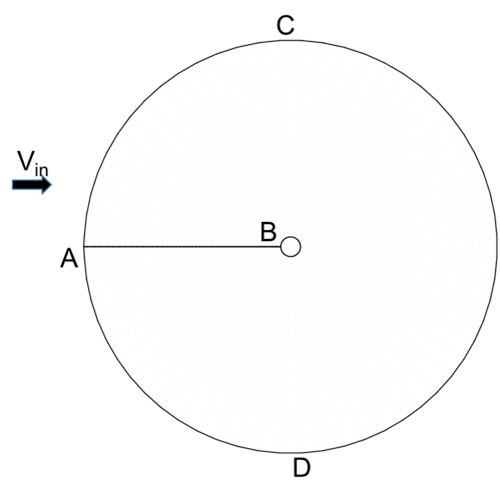
\includegraphics{figure/Рисунок1.png}
    \caption{Расчетная область O-топологии для расчета нестационарного обтекания цилиндра}
    \label{fig:my_label}
\end{figure}
Внутренняя окружность представляет собой поверхность обтекаемого цилиндра диаметром $d$, внешняя окружность – граница расчетной области диаметром $10d$. 

\subsubsection{Начальные и граничные условия}
На входе (дуги AC и AD) задается равномерный профиль скорости $v_x$ = 1. На границе CD задается постоянное нормированное давление $P$ = 0. Контур цилиндра – твердая стенка. AB – линия стыковки. (значения на границах, отмеченных как 1 и 3, должны совпадать.)

\subsubsection{Сетка}
\begin{figure}[H]
    \centering
    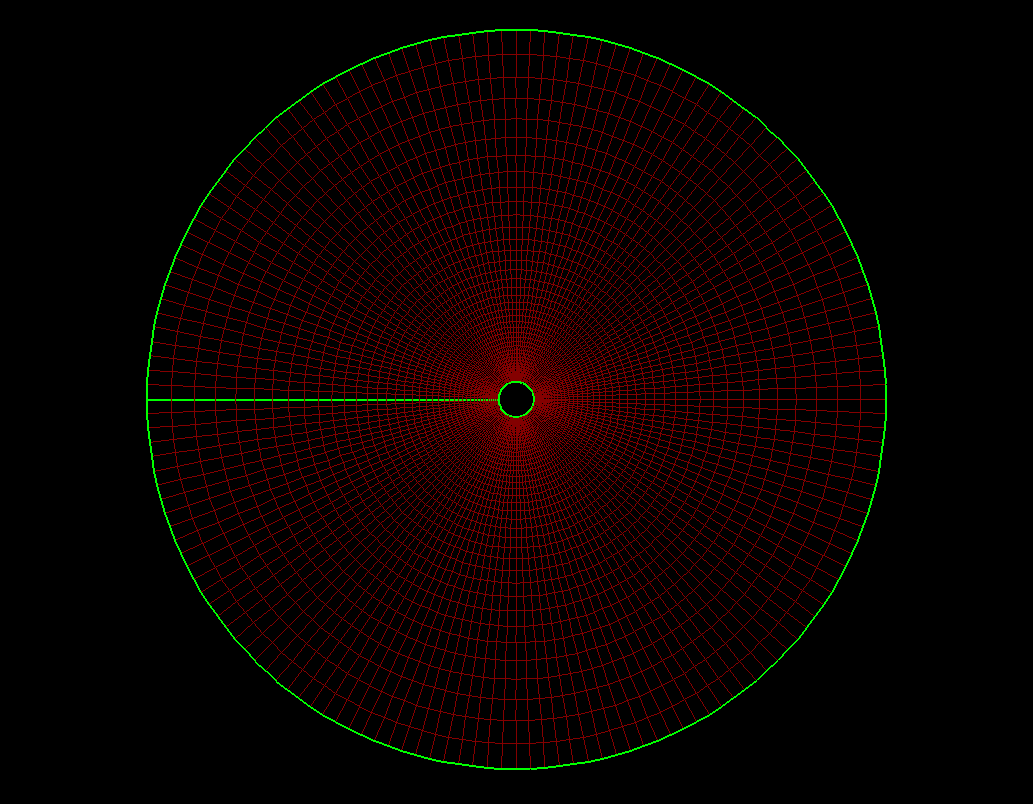
\includegraphics[scale=0.5]{figure/Setka.png}
    \caption{Расчетная сетка для расчета нестационарного обтекания цилиндра}
    \label{fig:my_labe2}
\end{figure}

\subsubsection{Решение}
\begin{figure}[H]
    \centering
    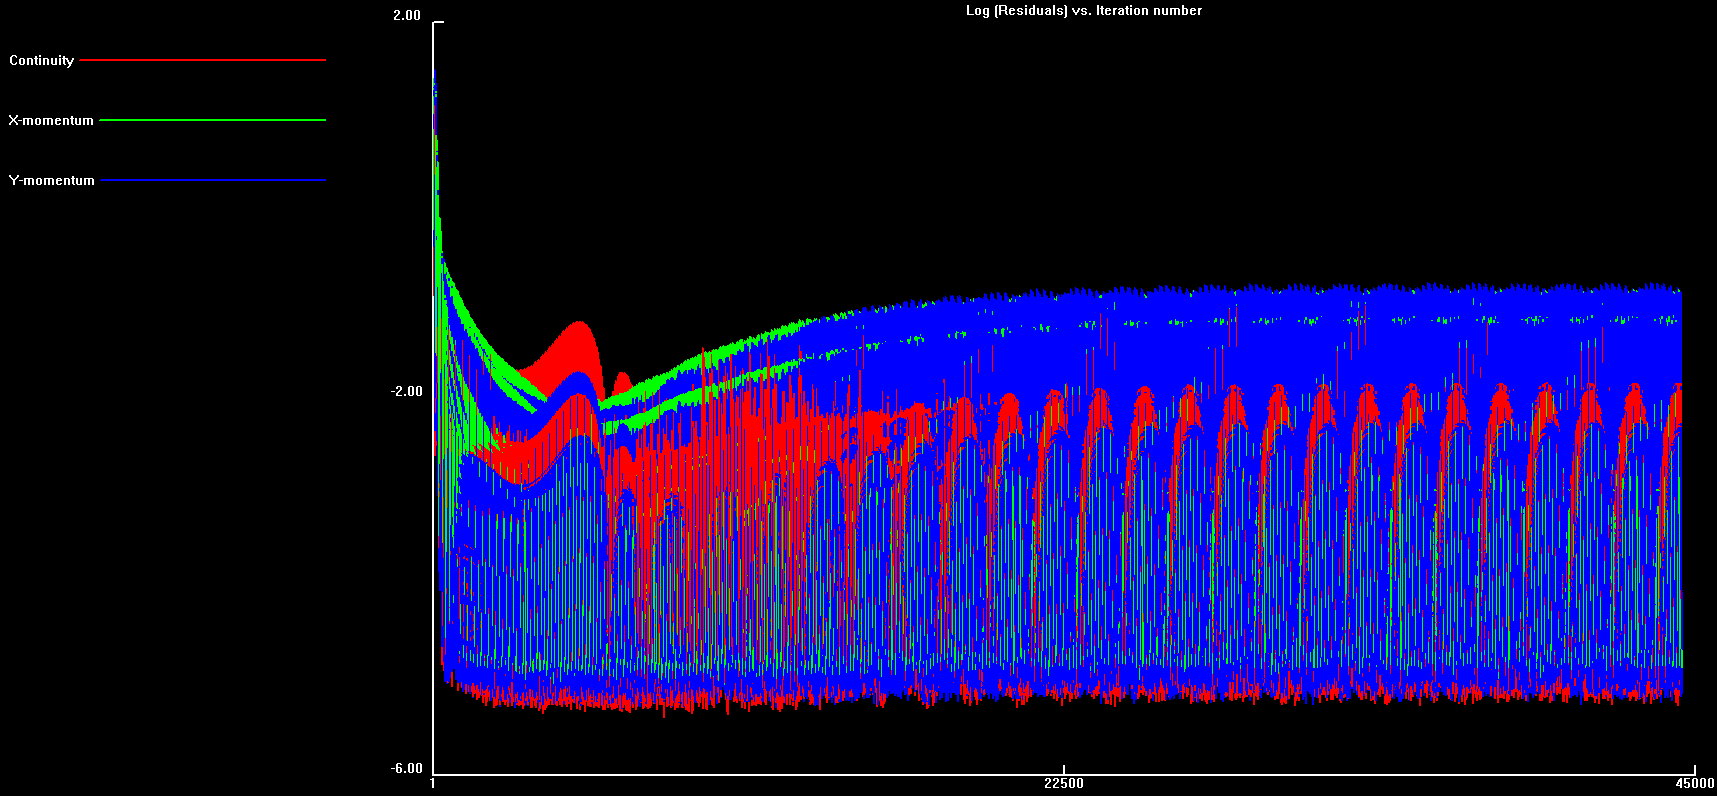
\includegraphics[scale=0.4]{figure/flos_t0.png}
    \caption{Эволюция во времени продольной и поперечной компонент вектора скорости и давления}
    \label{fig:my_labe3}
\end{figure}
На графике \ref{fig:my_labe3} показана зависимость невязки (расхождения) уравнений Навье-Стокса, уравнения неразрывности и уравнения энергии от числа итераций.Задача сразу решается как нестационарная. Это сделанно потому, что при исследуемом числе Рейнольдса(RE=80) не возникает достаточных возмущений для развития потока. Для внесения возмущений были добавлены следующие параметры: \\
$U_I_N_I_T = 1$  \\
$V_I_N_I_T = 0.1$  \\
 Нестационарную задачу решаем до тех пор, пока не будет достигнут статистически установившийся режим течения.

\subsection{Постпроцессинг}
\subsubsection{Эволюция вектора скорости и давления}

\begin{figure}[H]
    \centering
    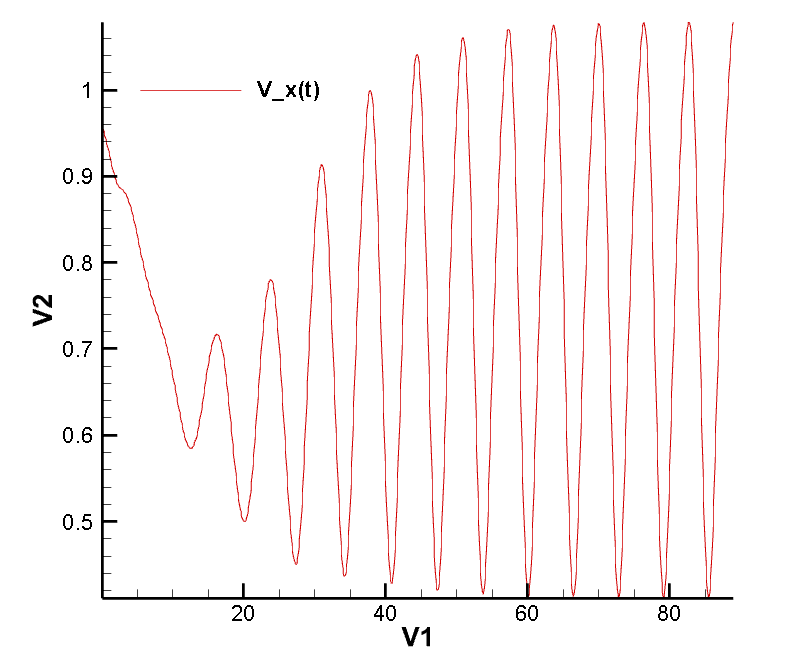
\includegraphics[scale=0.5]{figure/V_x(t).png}
    \caption{Изменение во времени x-компоненты вектора скорости $v_x$}
    \label{fig:my_labe5}
\end{figure}

\begin{figure}[H]
    \centering
    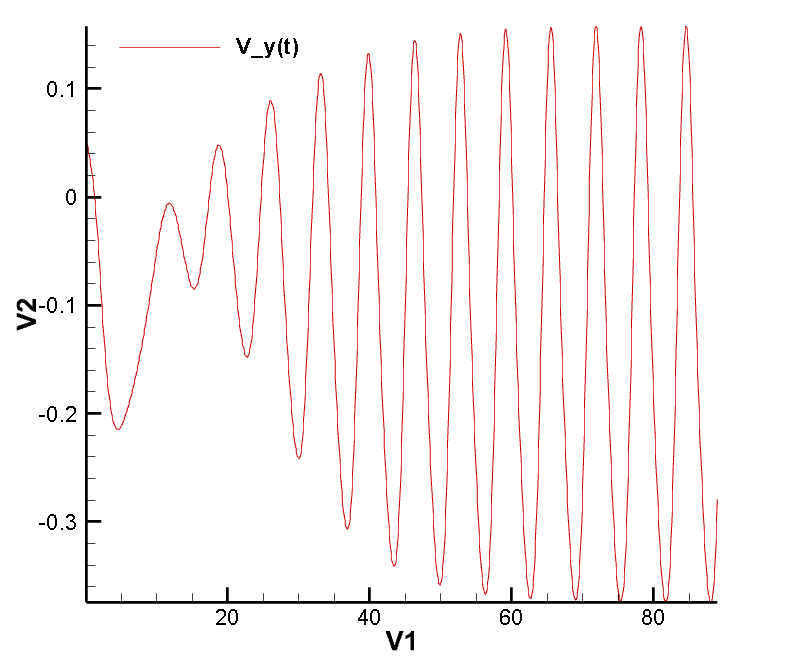
\includegraphics[scale=0.5]{figure/V_y(t).png}
    \caption{Изменение во времени y-компоненты вектора скорости $v_y$}
    \label{fig:my_labe4}
\end{figure}

\begin{figure}[H]
    \centering
    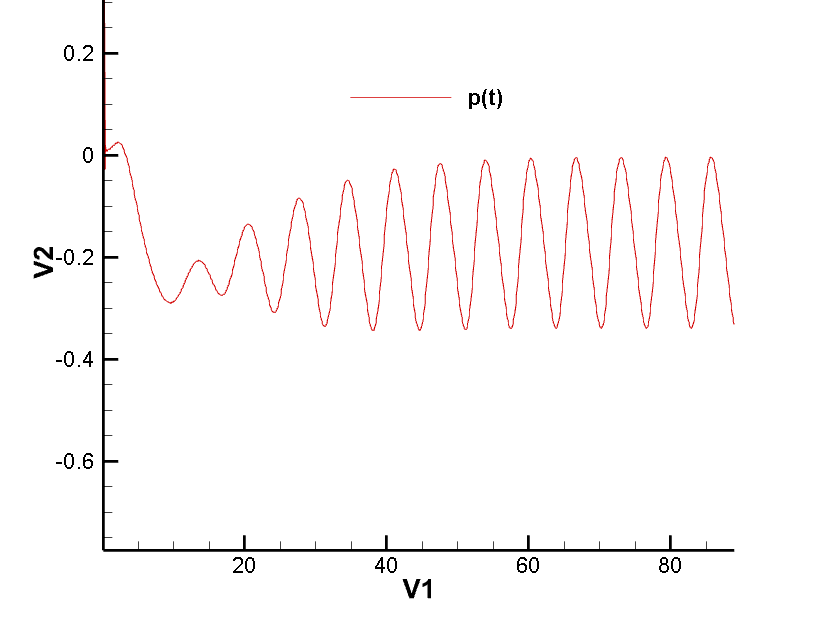
\includegraphics[scale=0.5]{figure/p(t).png}
    \caption{Изменение во времени давления $p$}
    \label{fig:my_labe6}
\end{figure}
Из графиков следует, что достигнут статистически периодический установившийся режим.

\newpage
\subsubsection{Поля параметров в различные моменты времени}
\subsubsubsection{Первый момент времени}
\begin{figure}[H]
    \centering
    \subfigure[Поле $v_x$]{
        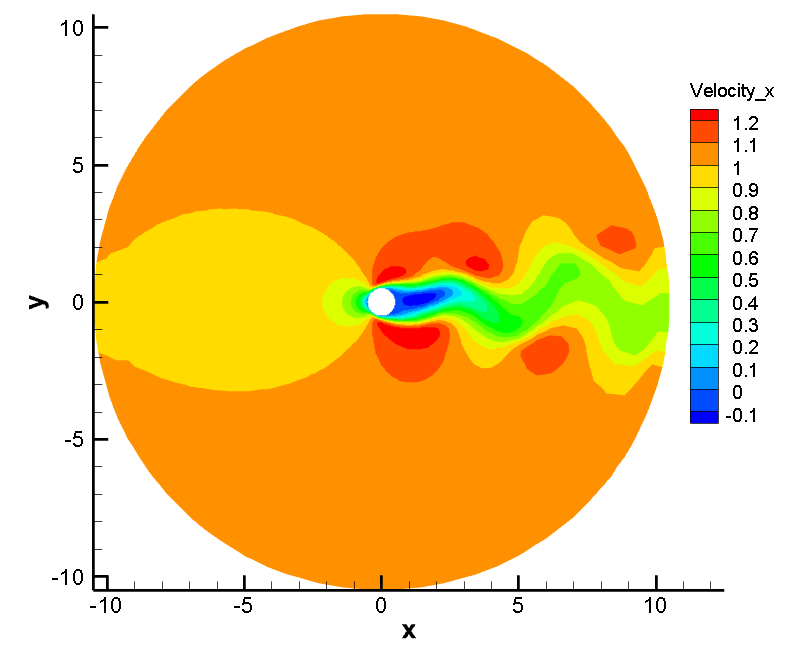
\includegraphics[scale=0.4]{figure/Velocity_x_t0.png}
        \label{fig:my_labe7_1}
    }
    \subfigure[Поле $v_y$]{
        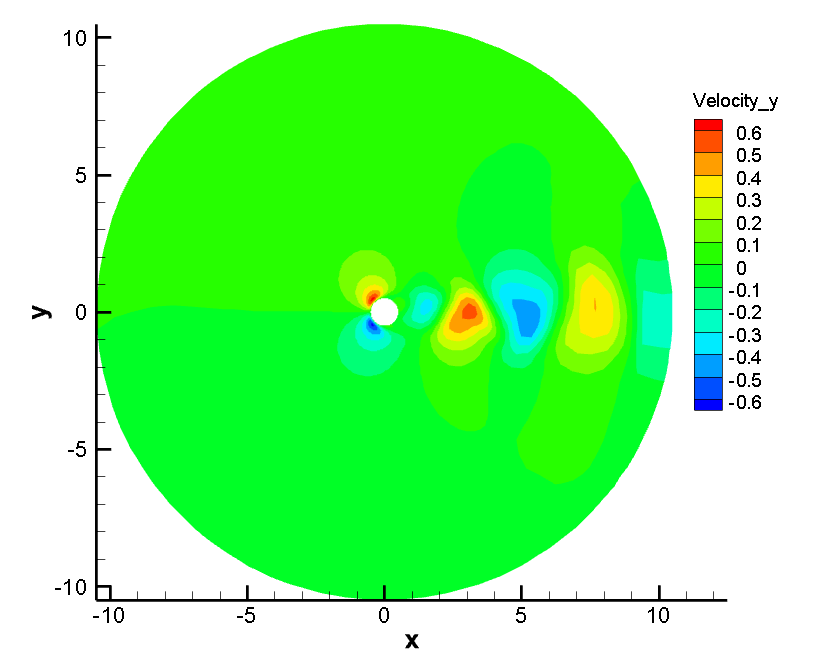
\includegraphics[scale=0.4]{figure/Velocity_y_t0.png}
        \label{fig:my_labe7_2}
    }
\end{figure}

\begin{figure}[H]
    \centering
    \subfigure[Поле модуля скорости $|v|$]{
        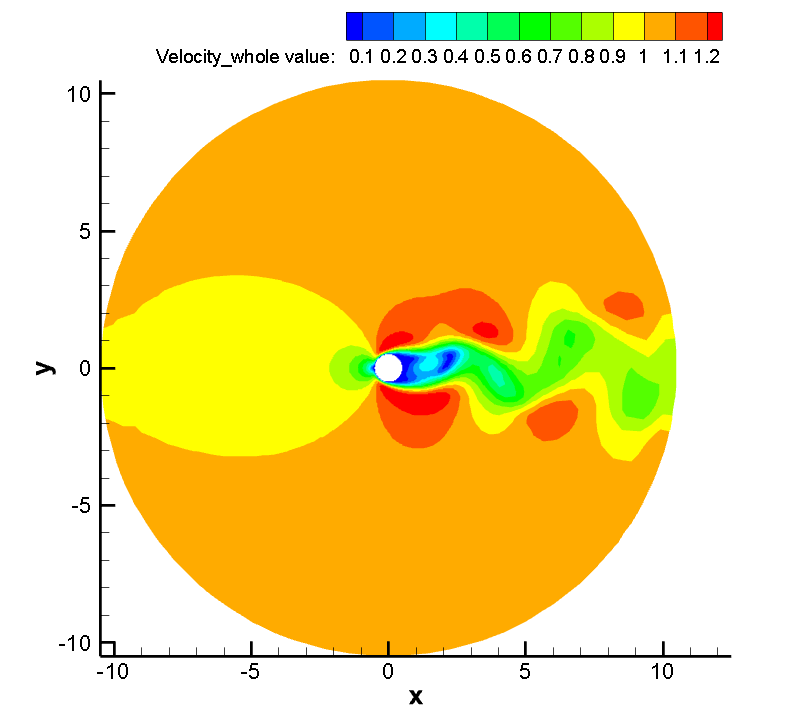
\includegraphics[scale=0.4]{figure/Velocity_whole_value_t0.png}
        \label{fig:my_labe7_3}
    }
    \subfigure[Поле давления $p$]{
        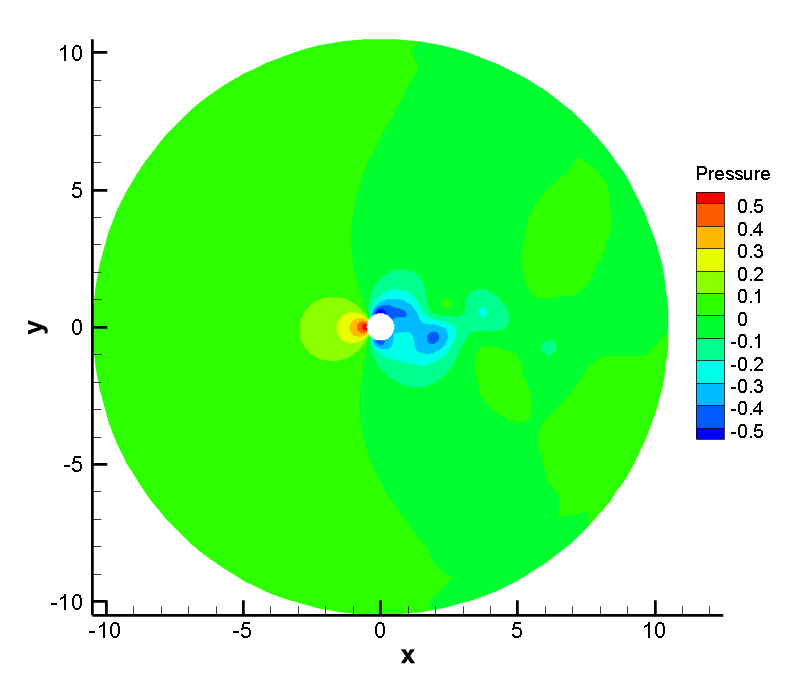
\includegraphics[scale=0.4]{figure/Pressure_t0.png}
        \label{fig:my_labe7_4}
    }
    \caption{Первый момент времени $t0$}
\end{figure}

Из картин в первый момент времени следует, что перед цилиндром скорость уменьшается, а давление увеличивается. Также образующаяся за цилиндром дорожка по своему виду совпадает на всех графиках.
За цилиндром образуются зоны низких скоростей, что также можно видеть из (\ref{fig:my_labe7_1}). Соответственно на (\ref{fig:my_labe7_4}) этим зонам соответствует зоны пониженного давления. 
В другие моменты времени получается схожая картина.

\newpage
\subsubsubsection{Второй момент времени}
\begin{figure}[H]
    \centering
    \subfigure[Поле $v_x$]{
        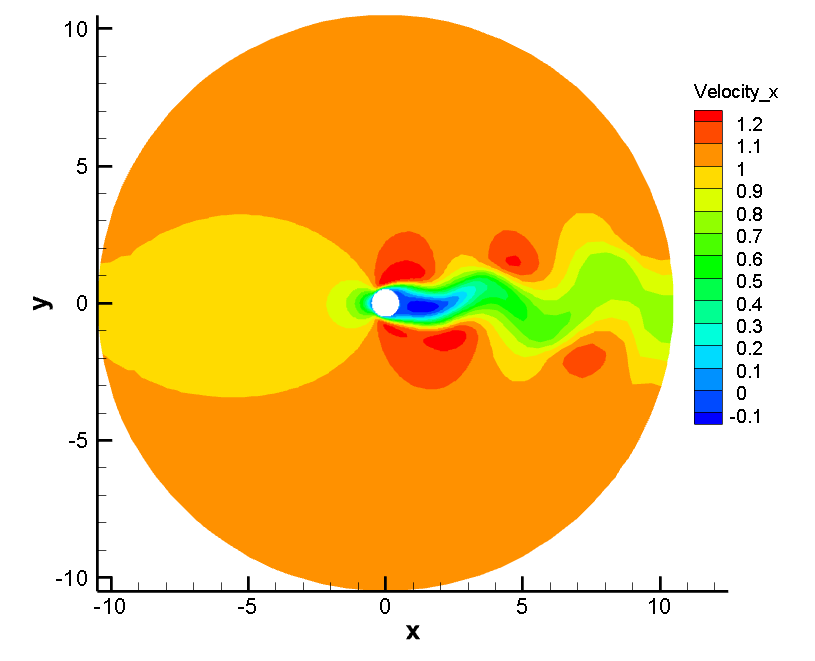
\includegraphics[scale=0.4]{figure/Velocity_x_t4.png}
        \label{fig:my_labe8_1}
    }
    \subfigure[Поле $v_y$]{
        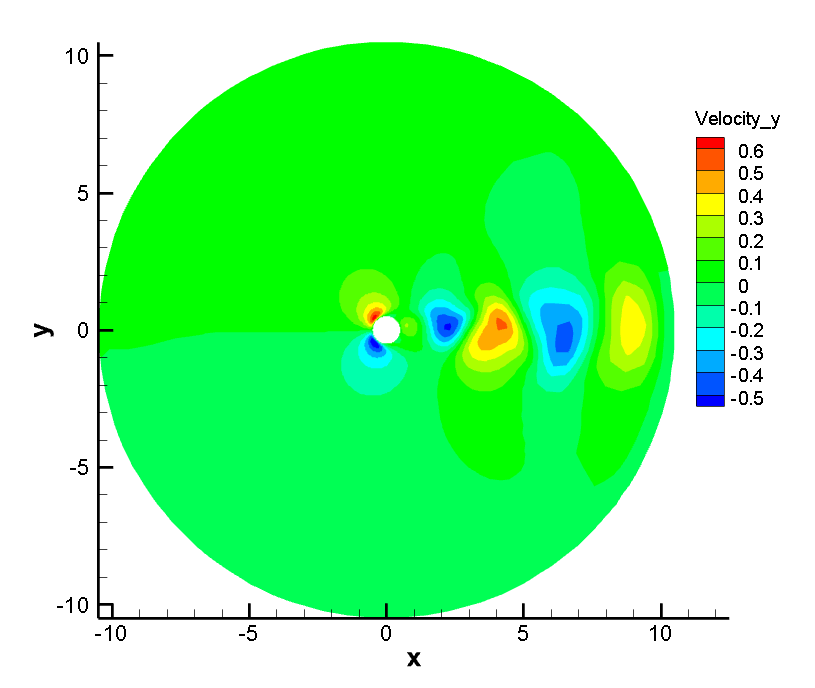
\includegraphics[scale=0.4]{figure/Velocity_y_t4.png}
        \label{fig:my_labe8_2}
    }
\end{figure}

\begin{figure}[H]
    \centering
    \subfigure[Поле модуля скорости $|v|$]{
        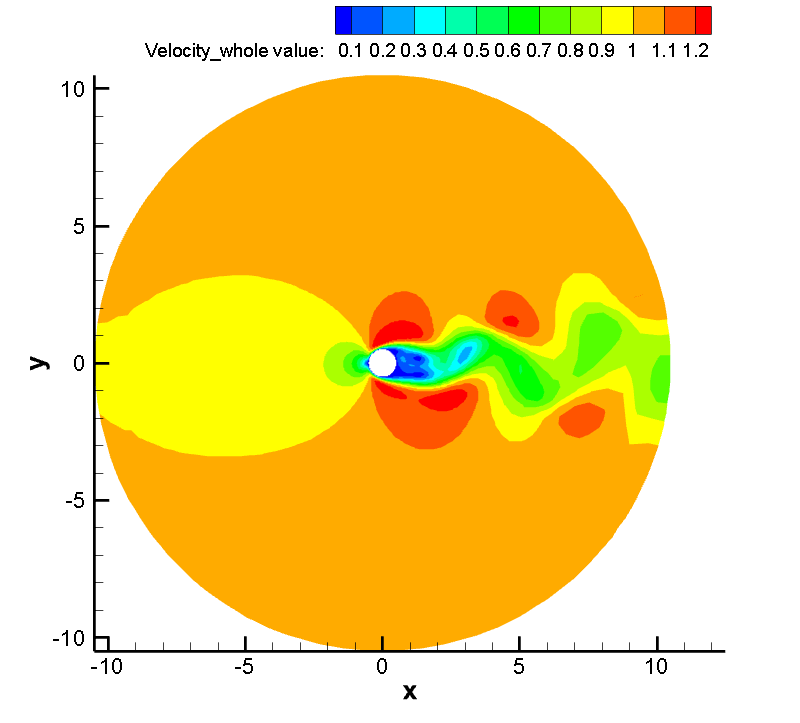
\includegraphics[scale=0.4]{figure/Velocity_whole_value_t4.png}
        \label{fig:my_labe8_3}
    }
    \subfigure[Поле давления $p$]{
        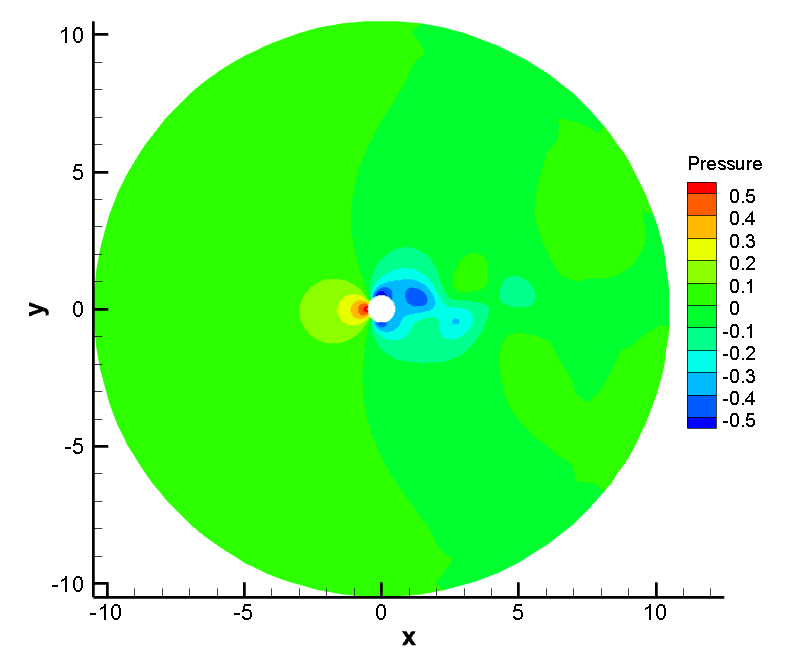
\includegraphics[scale=0.4]{figure/Pressure_t4.png}
        \label{fig:my_labe8_4}
    }
    \caption{Второй момент времени $t0 + T/4$}
\end{figure}

\newpage
\subsubsubsection{Третий момент времени}
\begin{figure}[H]
    \centering
    \subfigure[Поле $v_x$]{
        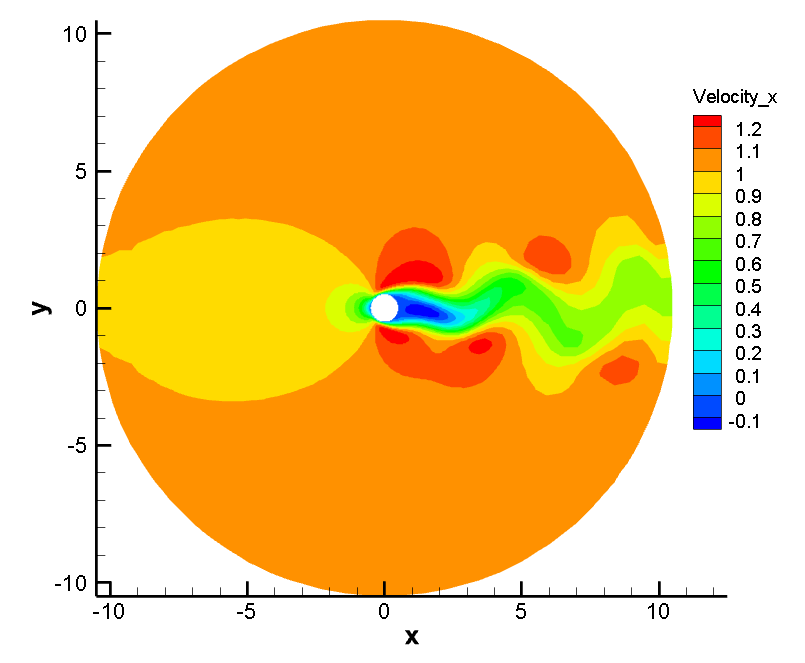
\includegraphics[scale=0.4]{figure/Velocity_x_t2.png}
        \label{fig:my_labe9_1}
    }
    \subfigure[Поле $v_y$]{
        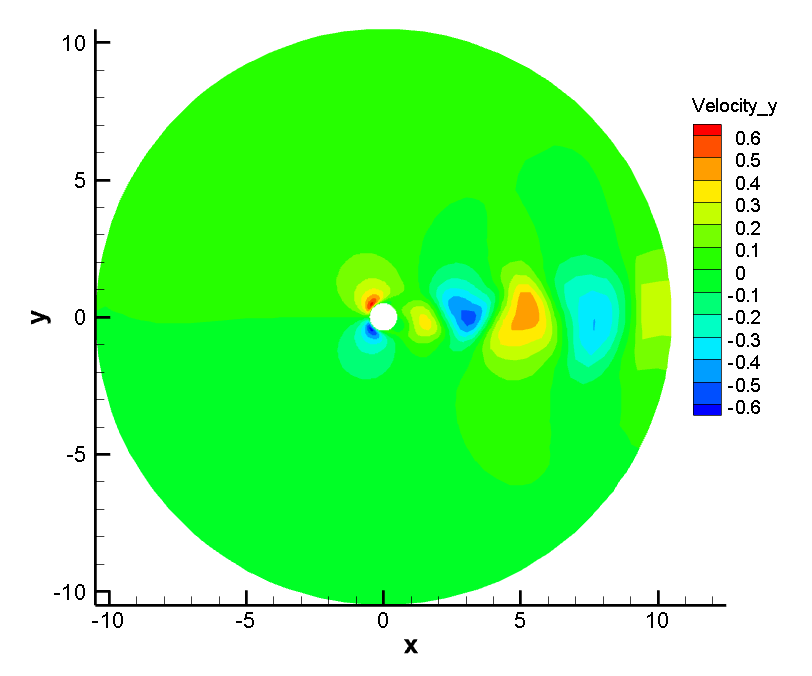
\includegraphics[scale=0.4]{figure/Velocity_y_t2.png}
        \label{fig:my_labe9_2}
    }
\end{figure}

\begin{figure}[H]
    \centering
    \subfigure[Поле модуля скорости $|v|$]{
        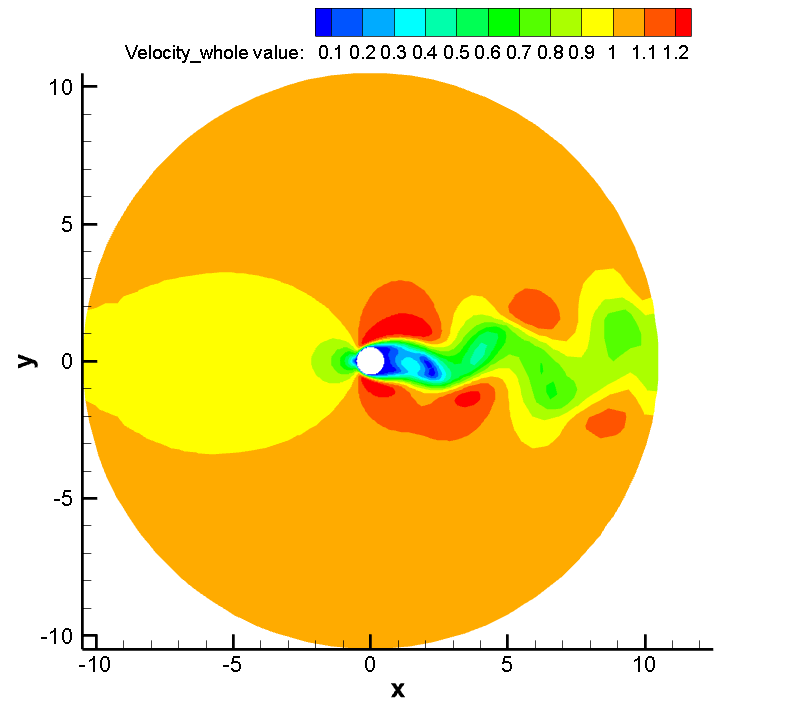
\includegraphics[scale=0.4]{figure/Velocity_whole_value_t2.png}
        \label{fig:my_labe9_3}
    }
    \subfigure[Поле давления $p$]{
        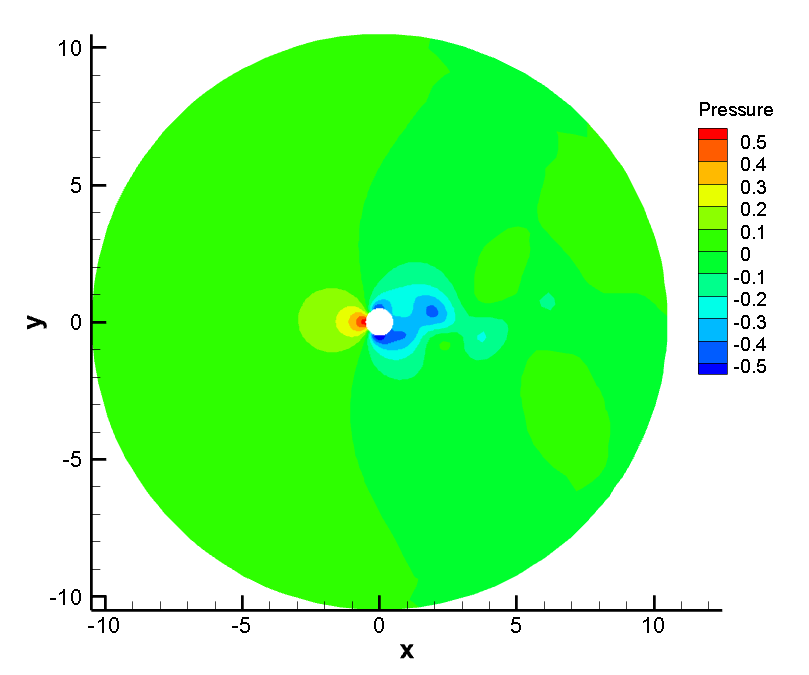
\includegraphics[scale=0.4]{figure/Pressure_t2.png}
        \label{fig:my_labe9_4}
    }
    \caption{Третий момент времени $t0 + T/2$}
\end{figure}

\newpage
\subsubsubsection{Четвертый момент времени}
\begin{figure}[H]
    \centering
    \subfigure[Поле $v_x$]{
        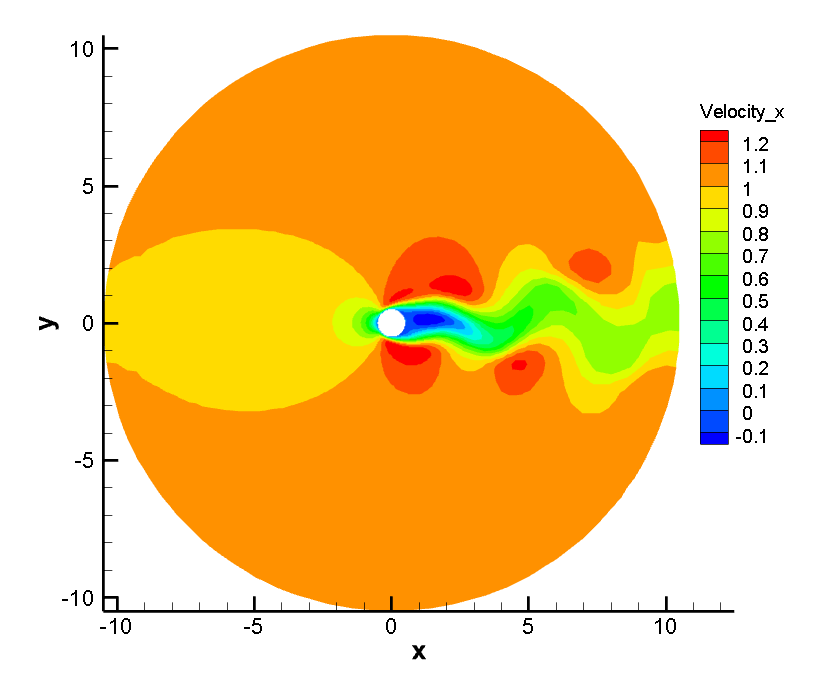
\includegraphics[scale=0.4]{figure/Velocity_x_3t4.png}
        \label{fig:my_labe10_1}
    }
    \subfigure[Поле $v_y$]{
        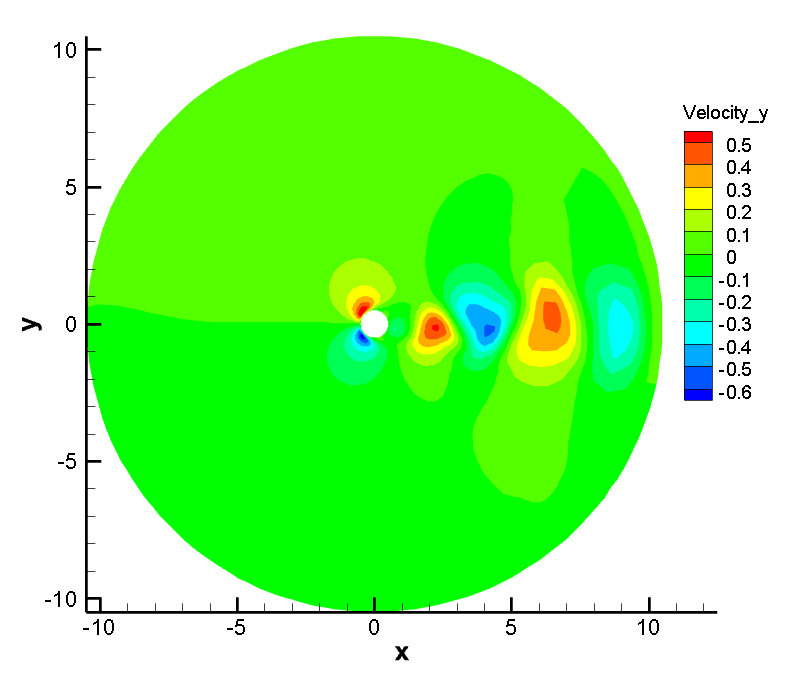
\includegraphics[scale=0.4]{figure/Velocity_y_3t4.png}
        \label{fig:my_labe10_2}
    }
\end{figure}

\begin{figure}[H]
    \centering
    \subfigure[Поле модуля скорости $|v|$]{
        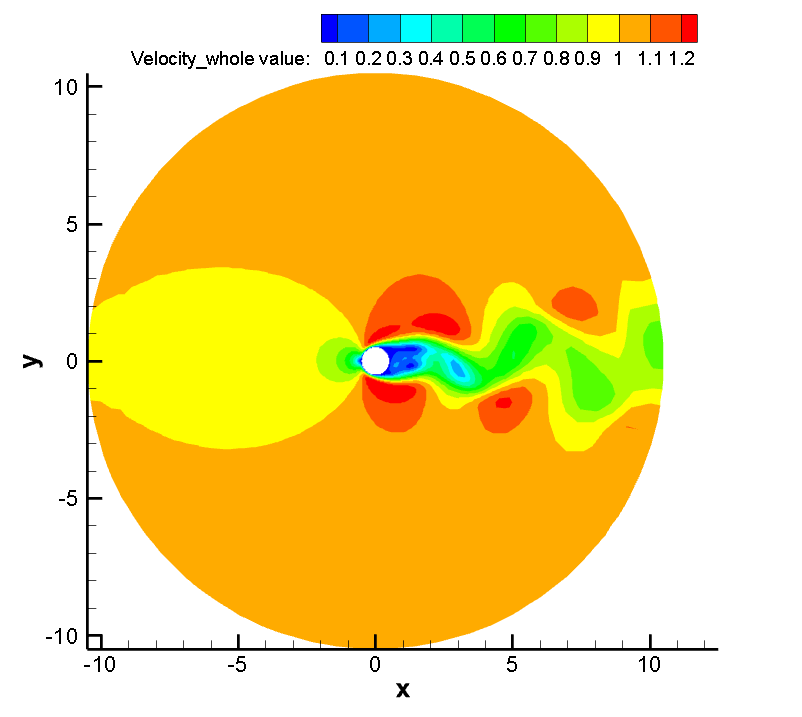
\includegraphics[scale=0.4]{figure/Velocity_whole_value_3t4.png}
        \label{fig:my_labe10_3}
    }
    \subfigure[Поле давления $p$]{
        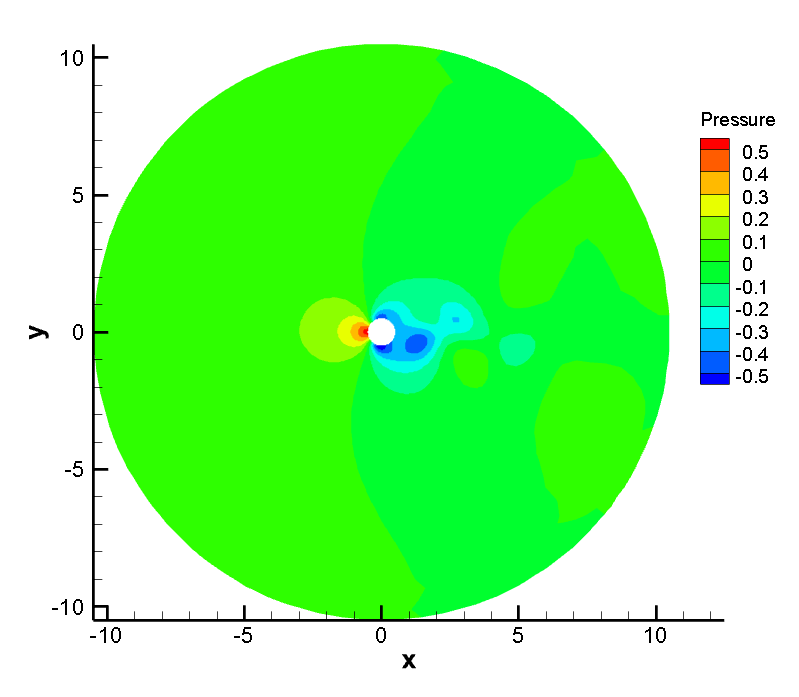
\includegraphics[scale=0.4]{figure/Pressure_3t4.png}
        \label{fig:my_labe10_4}
    }
    \caption{Четвертый момент времени $t0 + 3T/4$}
\end{figure}

\newpage
\subsubsection{Число Струхаля}
На рисунке (\ref{fig:my_labe4}) $t = [0, 55]$ – участок установления, $t > 55$- установившееся течение. Установившееся течение является периодическим с периодом $T = 82.6 - 76.3 = 6.3$ (по графику).
\begin{equation}
    Sh = \frac{L}{TV} = \frac{1}{T} = \frac{1}{6.3} = 0.1587
\end{equation}

\begin{figure}[H]
    \centering
    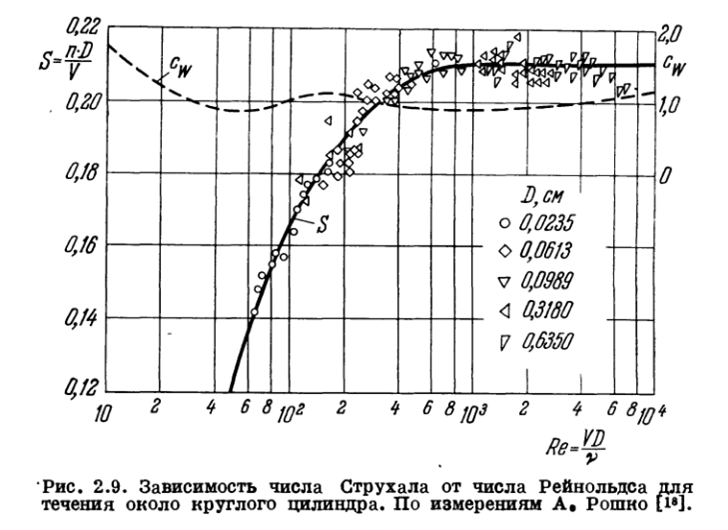
\includegraphics[scale=0.9]{figure/Рисунок11.png}
    \caption{Зависимость числа Струхаля от числа Рейнольдса}
    \label{fig:my_labe11}
\end{figure}

Полученное число Струхаля приблизительно равно числу, полученному в экспериментальных данных.
\end{document}